\documentclass[12pt]{beamer}
\usetheme{CambridgeUS}
\usepackage[utf8]{inputenc}
\usepackage[spanish]{babel}
\usepackage{amsmath}
\usepackage{amsfonts}
\usepackage{amssymb}
\usepackage{graphicx}
\usepackage{ragged2e}
\setbeamertemplate{navigation symbols}{} 
\author[Kevin García - Alejandro Vargas]{Kevin García 1533173 \newline Alejandro Vargas 1525953}
\title[Tarea 6: Selección de variables]{Tarea 6:Selección de variables}



%\setbeamercovered{transparent} 
%\setbeamertemplate{navigation symbols}{} 
%\logo{} 
%\institute{} 
%\date{} 
%\subject{} 
\begin{document}
\justify
\begin{frame}
\titlepage
\end{frame}

%\begin{frame}
%\tableofcontents
%\end{frame}
\begin{frame}
\frametitle{Introducción}
~\\En este trabajo se presentarán un método de selección de modelos que es el $R^2_{Ajustado}$ y dos algoritmos que son el Backward y el StepAIC, con ellos, se tratará de encontrar el mejor modelo posible para los 500 datos seleccionados de la base de datos 'Cadata', y se analizará el modelo obtenido. Además, se presentaran una serie de ventajas y desventajas de cada uno de los métodos y se formularan conclusiones a partir de los resultados arrojados.
\end{frame}

\begin{frame}
\frametitle{Introducción}
~\\En la mayoría de los problemas de construcción de modelos el analista tiene un grupo de regresores candidatos y debe determinar el subconjunto real de
regresores que debe usarse en el modelo. La definición de un subconjunto adecuado de regresores para el modelo es lo que se llama problema de selección de variables.
\end{frame}

\begin{frame}
\frametitle{Introducción}
~\\La construcción de un modelo de regresión que sólo incluya un subconjunto de los regresores disponibles implica dos objetivos contrapuestos: 1) Se desea que el modelo incluya tantos regresores como sea posible, para que el contenido de información en ellos pueda influir sobre el valor predicho de y. 2) Se desea que el modelo incluya los menos regresores que sea posible, porque la varianza de la predicción $\hat{y}$ aumenta a medida que aumenta la cantidad de regresores. También, mientras más regresores haya en un modelo, los costos de recolección de datos y los de mantenimiento de modelo serán mayores. Entonces, con la selección de variables se trata de encontrar el punto medio entre los dos objetivos anteriores, logrando hallar así la 'mejor' recta de regresión.
\end{frame}

\begin{frame}
\frametitle{Modelo Completo}
~\\El modelo completo con todas las variables bajo el cual se está trabajando es:

~\\$$\hat{ValorMediano} = 57720.52 + 24261.20IngresoMediano +$$
$$3443.94EdadMediana + 19.09TotalHabitaciones$$
$$ - 67.72TotalDormitorios - 121.66Poblacion +315.92Hogares $$
\end{frame}

\begin{frame}
\frametitle{Descripción de criterios y algoritmos de selección}
\begin{itemize}
\item $R^2_{Ajustado}$: Usando el método del $R^2_{Ajustado}$, se deben realizar todas las posibles combinaciones de modelos a partir de las variables que tenemos, y seleccionar el modelo que tenga mayor $R^2_{Ajustado}$. Este método surgió como una alternativa al método del coeficiente de determinación $R^2$, ya que el $R^2$ no tiene en cuenta la cantidad de parámetros del modelo, es decir, este siempre aumenta a medida que se ingresa una nueva variable al modelo.
~\\El $R^2_{Ajustado}$ se define como:
$$R^2_{Adj}=1-\frac{N-1}{N-k-1}(1-R^2)$$ 
~\\Donde N es el tamaño de muestra y k es la cantidad de parámetros del modelo y $R^2=\frac{SCR_{D}}{SCT_{D}}=\frac{\sum\limits_{i=1}^{n}(\hat{y_{i}}-\bar{y})^2}{\sum\limits_{i=1}^{n}(y_{i}-\bar{y})^2}$.
\end{itemize}
\end{frame}

\begin{frame}
\frametitle{Descripción de criterios y algoritmos de selección}
\begin{itemize}
\item Backward (selección hacia atrás): Como su nombre lo indica se comienza por considerar incluidas en el modelo teórico a todas las variables disponibles y se van eliminando del modelo de una en una según su capacidad explicativa. Para esto,  la primera variable que se elimina es aquella que presenta un menor coeficiente de correlación parcial  con la variable dependiente o lo que es equivalente, un menor valor del estadístico W y así sucesivamente hasta llegar a una situación en la que la eliminación de una variable más suponga un descenso demasiado acusado en el coeficiente de determinación.
\end{itemize}
\end{frame}

\begin{frame}
\frametitle{Descripción de criterios y algoritmos de selección}
~\\Algoritmo:
\begin{itemize}
\item[1.] Se toma el modelo completo (con todas las variables disponibles)
\item[2.] Se obtiene la reducción de la variación de los datos para cada variable, denotado por, $R(\vec{\beta_{1}}|\vec{\beta_{2}})$ (es la suma de cuadrados de la regresión del modelo completo menos la suma de cuadrados de la regresión del modelo reducido).
\item[3.] Se selecciona como candidata a salir, aquella variable cuya reducción sea la más pequeña.
\item[4.] Se realiza una prueba de significancia para el coeficiente $\beta$ correspondiente a la variable candidata a salir. Si esta no se rechaza, estaríamos concluyendo que $\beta=0$, y por lo tanto la variable sale del modelo.
\end{itemize}
\end{frame}

\begin{frame}
\frametitle{Descripción de criterios y algoritmos de selección}
\begin{itemize}
\item[5.] Se toma como modelo completo al modelo resultante sin la variable excluida del item anterior y se hace el mismo procedimiento. 
\item[6.] El algoritmo se detiene cuando la prueba de significancia se rechace, y se toma como modelo final, el modelo completo hasta esa prueba de significancia.
\end{itemize}
\end{frame}

\begin{frame}
\frametitle{Descripción de criterios y algoritmos de selección}
\begin{itemize}
\item StepAIC (selección paso a paso con el criterio de información de Akakike (AIC)): Consiste en una combinación entre el Forward y el Backward. En el primer paso se procede como en el método forward pero a diferencia de éste en el que cuando una variable entra en el modelo ya no vuelve a salir, en el procedimiento stepwise es posible que la inclusión de una nueva variable haga que otra que ya estaba en el modelo resulte redundante y sea ``expulsada'' de él.
Cuando se aplica este tipo de procedimientos tenemos que tener en cuenta cual sería la condición para suprimir o incluir un término. Para ello podemos considerar dos criterios: criterios de significación del término y criterios de ajuste global.
\end{itemize}
\end{frame}

\begin{frame}
\frametitle{Descripción de criterios y algoritmos de selección}
\begin{itemize}
\item[-] Criterios de significación: En un método backward se suprimirá el término que resulte menos significativo, y en un método forward se añadirá el término, que al añadirlo al modelo resulte más significativo. Un criterio de significación puede ser la significación de cada coeficiente (SCR)
\item[-] Criterios globales: En vez de usar la significación de cada coeficiente, podemos basarnos en un criterio global, una medida global de cada modelo, de modo que tenga en cuenta el ajuste y el exceso de parámetros. Escogeremos el modelo cuya medida global sea mejor. Como criterios destacamos el Criterio de Información de Akaike (AIC) y el Criterio de Información de Bayes (BIC). Se trata de buscar un modelo cuyo AIC o BIC sea pequeño, ya que en ese caso habría una verosimilitud muy grande y pocos parámetros.
\end{itemize}
\end{frame}

\begin{frame}
\frametitle{Descripción de criterios y algoritmos de selección}
Para este caso tenemos como algoritmo el Stepwise, con un criterios global de Información de Akaike (AIC). Como ya se mencionó se desea elegir el modelo que presente menor AIC.
~\\Algoritmo:
\begin{itemize}
\item[1.] Se toma como modelo inicial, solo con el intercepto, es decir, un modelo de la forma $Y=\beta_{0}$ y se calcula el AIC correspondiente
\item[2.] Se ajustan los modelos para cada una de las variables disponibles, es decir, un modelo de la forma $=\beta_{0}+\beta_{1}X_{i}$ en nuestro caso $i=1,2,3,4,5,6$. Para cada uno de ellos se calcula el AIC e ingresa al modelo la variable cuyo AIC sea menor y a su vez debe ser menor que el modelo inicial.
\end{itemize}
\end{frame}

\begin{frame}
\frametitle{Descripción de criterios y algoritmos de selección}
\begin{itemize}
\item[3.] Se toma el nuevo modelo como inicial y se hace el mismo procedimiento. Se calcula su AIC y se ajustan los modelos para cada una de las variables disponibles (modelos de la forma $Y=\beta_{0}+\beta_{1}X_{i}+\beta_{2}X_{j}$), incluso para la variable que entró se calcula un modelo sin ella (modelo de la forma $Y=\beta_{0}$ ). Se calcula nuevamente el AIC para cada uno de ellos y se ingresa la variable cuyo modelo tenga un AIC menor y este a su vez sea menor que el del modelo inicial, en caso de que el AIC menor corresponda al modelo en el cual se quita la variable que entró, esta sale del modelo.
\item[4.] Se procede de la misma manera hasta que el AIC de las variables a entrar o a salir ninguno sea menor que el AIC del modelo inicial.
\item[5.] De esta manera tendríamos un modelo final con todas las variables que ingresaron.
\end{itemize}
\end{frame}

\begin{frame}
\begin{figure}[h]
  \centering
  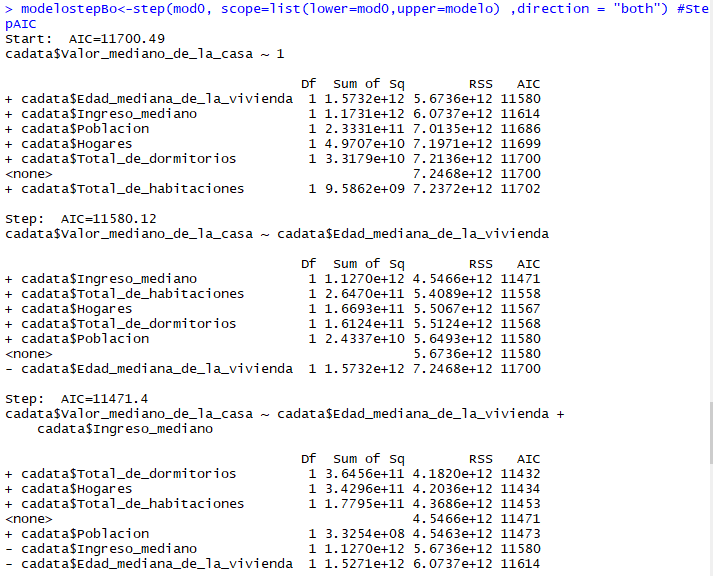
\includegraphics[scale=0.5]{imagenes/AIC1.png}
\end{figure}
\end{frame}

\begin{frame}
\begin{figure}[h]
  \centering
  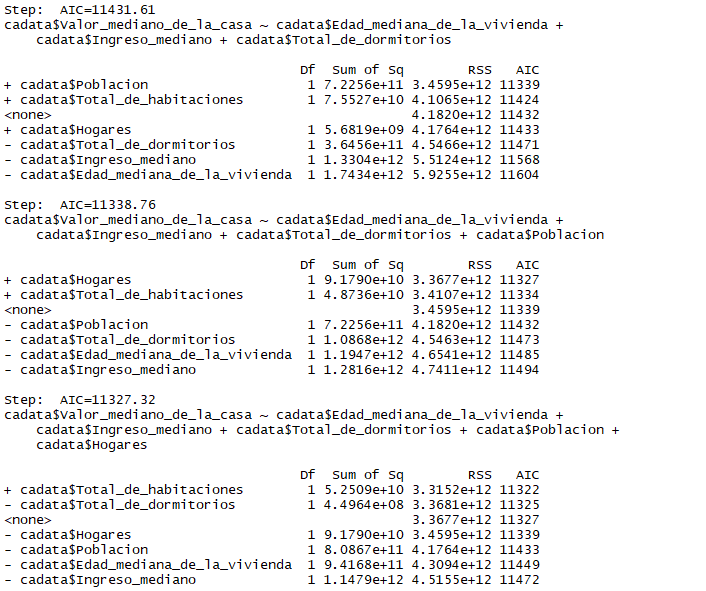
\includegraphics[scale=0.5]{imagenes/AIC2.png}
\end{figure}
\end{frame}

\begin{frame}
\begin{figure}[h]
  \centering
  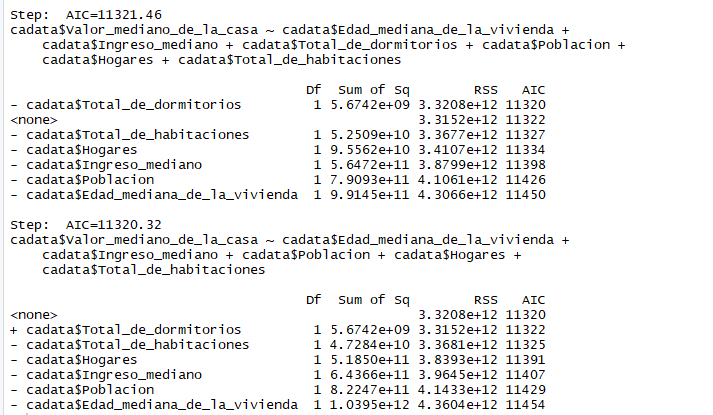
\includegraphics[scale=0.55]{imagenes/AIC3.png}
\end{figure}
\end{frame}

\begin{frame}
\frametitle{Análisis del modelo seleccionado}
~\\ Los modelos seleccionados por el método del $R^2_{Ajustado}$ y por los algoritmos Backward y StepAIC con el paquete fueron exactamente el mismo, es decir, los tres métodos nos arrojaron las mismas variables seleccionadas que fueron Ingreso mediano, Edad mediana, Total de habitaciones, Población y Hogares (solo eliminaron la variable Total de Dormitorios).
~\\Ese modelo fue:
~\\$\hat{ValorMediano}=52921.68807+24923.24378 IngresoMediano$
$$+ 3484.16424 EdadMediana+17.58804 TotalHabitaciones$$
$$-118.65234 Poblacion +243.26500 Hogares$$
\end{frame}

\begin{frame}
\frametitle{Análisis del modelo seleccionado}
\begin{figure}[h]
  \centering
  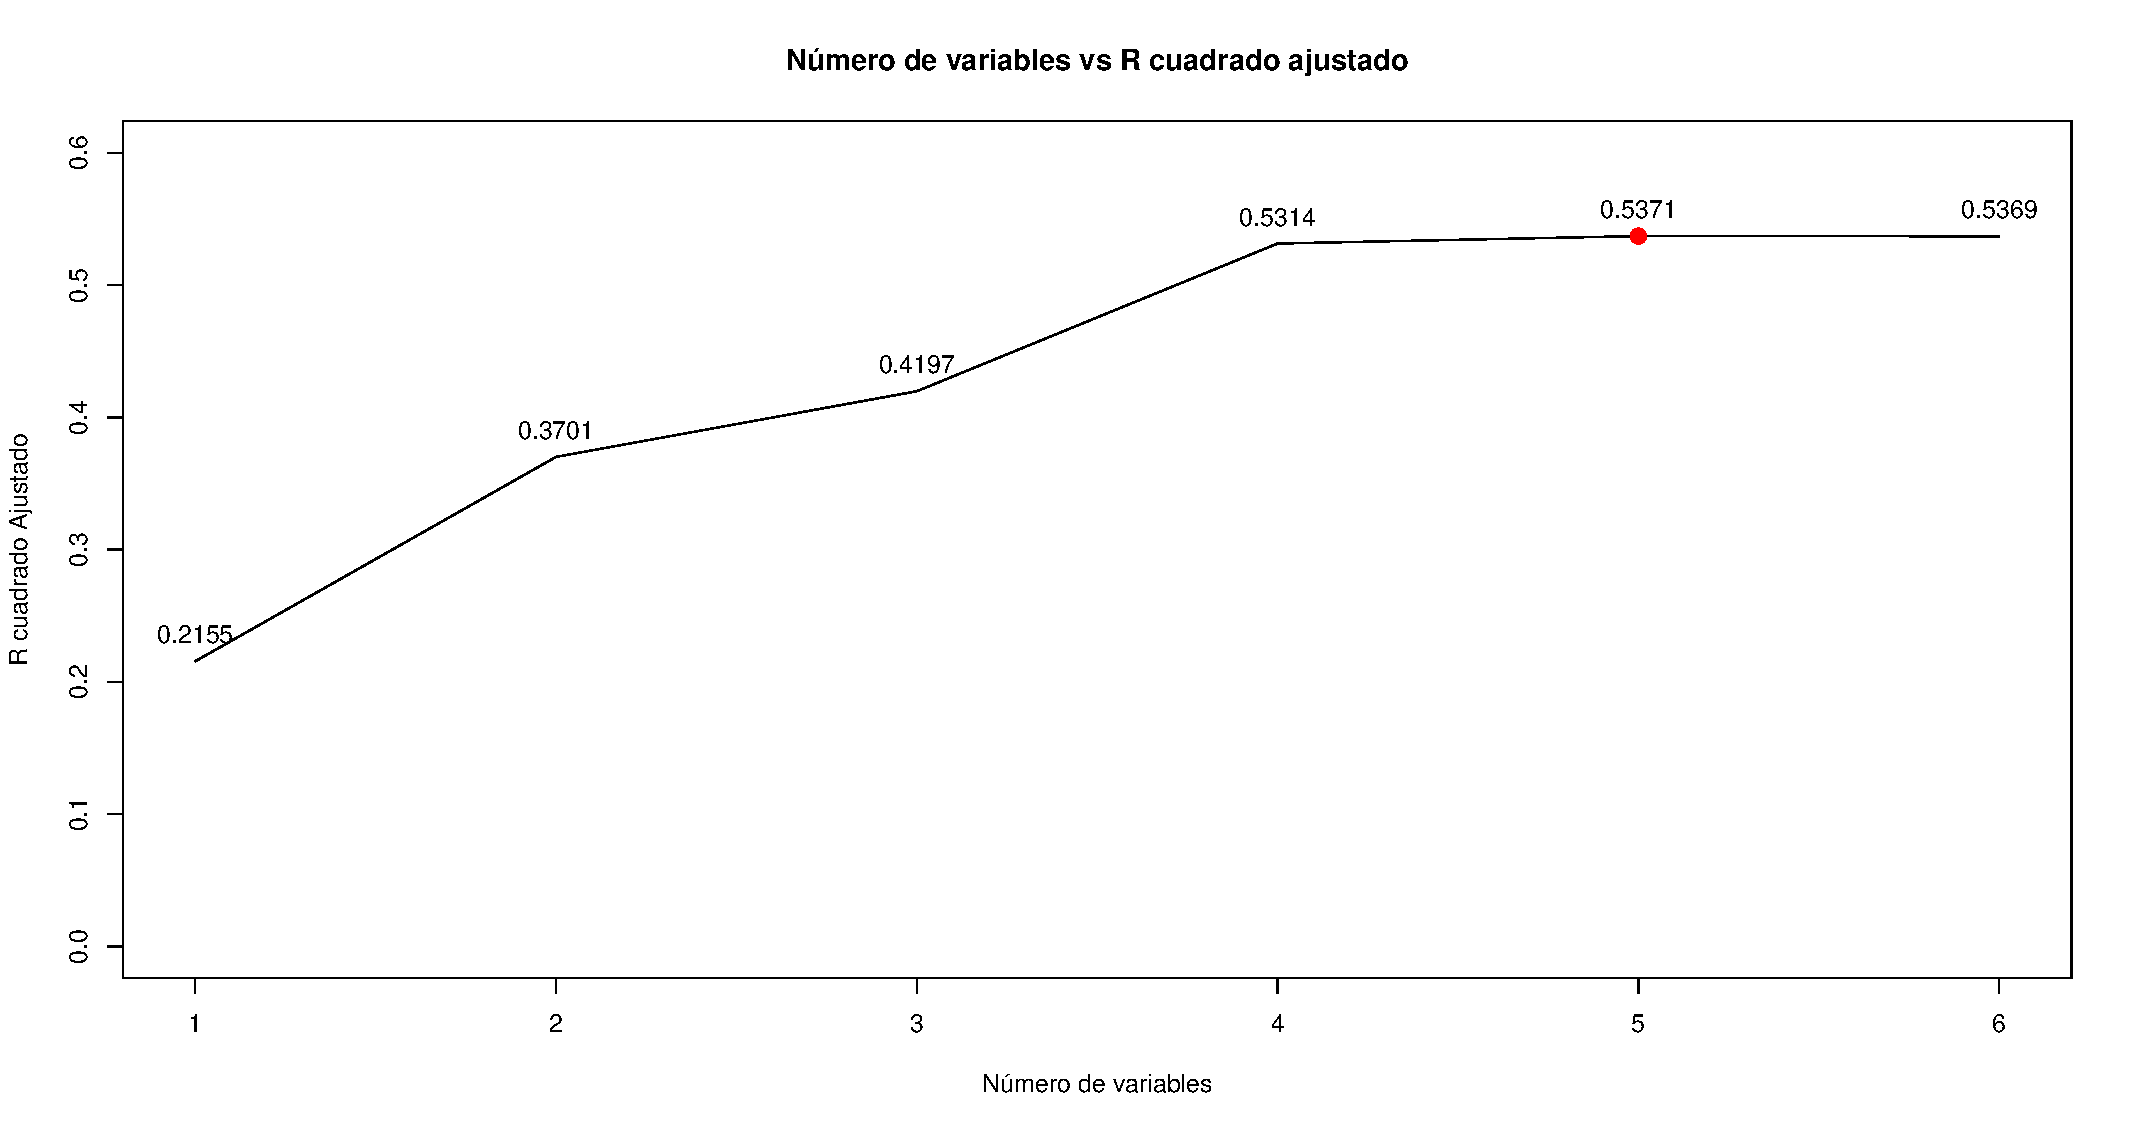
\includegraphics[scale=0.3]{imagenes/r2.pdf}
  \caption{Gráfico de número de variables contra $R^2_{Ajustado}$}\label{figura1}
\end{figure}
\end{frame}

\begin{frame}
\frametitle{Análisis del modelo seleccionado}
~\\En la imagen anterior podemos ver la representación gráfica del método del $R^2_{Ajustado}$, los 6 modelos representados correspondientes a 1,2,3,4,5 y 6 variables, son los mejores modelos que se pueden construir con tal número de variables con respecto al $R^2_{Ajustado}$, es decir, la gráfica muestra el $R^2_{Ajustado}$ del mejor modelo con cada número de variables pero en el trasfondo ya se han ajustado todos los posibles modelos por cantidad de variables. Lo que hace el método es elegir al modelo con el $R^2_{Ajustado}$ más alto, por lo cuál elige al mejor modelo con 5 variables que es el mencionado anteriormente.
\end{frame}

\begin{frame}
\frametitle{Análisis del modelo seleccionado}
~\\Para el respectivo análisis del modelo, tenemos las siguientes dos tablas:
\begin{center}
\begin{tabular}{|ccccc|}
\hline 
 & Estimación & Std. Error & Valor t & Pr($>|t|$) \\ 
\hline 
Intercepto & 52921.688 & 17525.287 & 3.020 & 0.00266 \\ 
Ingreso Mediano & 24923.244 & 2547.044 & 9.745 & $<2e-16$ \\  
Edad Mediana & 3484.164 & 280.184 & 12.435 & $<2e-16$ \\ 
Total Habitaciones & 17.588 & 6.632 & 2.652 & 0.00826 \\ 
Población & -118.652 & 10.727 & -11.061 & $<2e-16$ \\  
Hogares & 243.265 & 27.699 & 8.782 & $<2e-16$ \\ 
\hline 
\end{tabular} 
\end{center}
\begin{center}
\begin{tabular}{|c|c|c|c|c|}
\hline 
$\hat{\sigma}$ & $R^2$ & $R^2_{Ajustado}$ & Estadístico F & P Valor \\ 
\hline 
81990 & 0.5417 & 0.5371 & 116.8 & $<2.2e-16$ \\ 
\hline 
\end{tabular} 
\end{center}
\end{frame}

\begin{frame}
\frametitle{Análisis del modelo seleccionado}
~\\Podemos ver en las dos tablas anteriores que todas las variables incluidas son significativas (el p valor de cada una de ellas es menor a 0.05) y por tanto, el modelo en general también es significativo. Además, tanto el $R^2$ como el $R^2_{Ajustado}$ son casi los mismos que los del modelo completo (0.5425 y 0.537 respectivamente), por lo tanto podríamos concluir que la inclusión de la variable Total de Dormitorios no daba un aporte adicional a la explicación del valor mediano de la vivienda. Adicionalmente, la desviación del modelo a los datos disminuyó un poco (de 82000 del modelo completo a 81990 en el modelo con selección de variables), por lo cuál se podría decir que la variable excluida en este problema en particular solo servía para aumentar los costos de recolección de datos y para aumentar la desviación del modelo y en general, las desviaciones de los valores ajustados.
\end{frame}

\begin{frame}
\frametitle{Ventajas y desventajas de los algoritmos y métodos utilizados}
~\\Como ventajas o desventajas para el método y para los dos algoritmos tenemos las siguientes:
\begin{itemize}
\item $R^2_{Ajustado}$
~\\Desventajas:
\begin{itemize}
\item[1.] Es el mas tedioso de todos en cuanto a cálculos, ya que toca ajustar todos los posibles modelos para todas las posibles combinaciones de variables, es decir, se deben ajustar todos los posibles modelos (6) para una variable, todos los posibles (15) para 2 variables, y así sucesivamente. En total en este caso son $6 \choose 1$ + $ 6 \choose 2$ + $ 6\choose 3$ +...+ $6\choose 6$ $=63$ modelos que se deben ajustar.
\end{itemize}
\end{itemize}
\end{frame}

\begin{frame}
\frametitle{Ventajas y desventajas de los algoritmos y métodos utilizados}
\begin{itemize}
\item[2.] El criterio de selección es el más débil, ya que solo usamos el $R^2_{Ajustado}$ para decidir, y está demostrado que es mejor criterio el AIC porque no solo penaliza por la cantidad de parámetros o la complejidad del modelo, sino también por la capacidad predictiva que este tiene.
\item[3.] Al seleccionar al modelo con mayor $R^2_{Ajustado}$ no toma en cuenta si en realidad esas diferencias entre $R^2$ es significativa, es decir, un modelo con 4 variables como nos sucedió puede tener un $R^2_{Ajustado}$ de 0.5314 y el modelo con 5 tener un $R^2_{Ajustado}$ de 0.5371, y puede no valer la pena incluir la quinta variable para un aumento tan insignificante en el $R^2_{Ajustado}$, ya que eso implicaría mas costos y trabajo en la medición de ella.   
\end{itemize}
\end{frame}

\begin{frame}
\frametitle{Ventajas y desventajas de los algoritmos y métodos utilizados}
~\\ Ventajas:
\begin{itemize}
\item[1.] La regla de decisión y de selección es muy sencilla de calcular y de aplicar.
\end{itemize}
\end{frame}

\begin{frame}
\frametitle{Ventajas y desventajas de los algoritmos y métodos utilizados}
\begin{itemize}
\item Algoritmo Backward
~\\ Desventajas:
\begin{itemize}
\item[1.] Tiene la desventaja de necesitar mucha capacidad de cálculo si la cantidad de variables regresoras es grande.
\item[2.] Puede conducir a problemas de multicolinealidad si las variables están relacionadas, ya que esta no evalúa la salida de posibles variables ante la entrada de otras.
\end{itemize}
\end{itemize}
\end{frame}

\begin{frame}
\frametitle{Ventajas y desventajas de los algoritmos y métodos utilizados}
~\\ Ventajas:
\begin{itemize}
\item[1.] No elimina variables significativas para el modelo.
\item[2.] No necesita que se defina un término como umbral, ni que se defina la cantidad de variables a seleccionar.
\end{itemize}
\end{frame}

\begin{frame}
\frametitle{Ventajas y desventajas de los algoritmos y métodos utilizados}
\begin{itemize}
\item Algoritmo StepAIC
~\\ Desventajas:
\begin{itemize}
\item[1.] La única desventaja que logramos encontrar en este método es la gran cantidad de cálculos que se deben hacer, ya que se tienen que ajustar demasiados modelos y encontrar su AIC correspondiente.
\end{itemize}
\end{itemize}
\end{frame}

\begin{frame}
\frametitle{Ventajas y desventajas de los algoritmos y métodos utilizados}
~\\ Ventajas:
\begin{itemize}
\item[1.] Usa como criterio de selección el criterio de información de Akaike (AIC), el cuál es un criterio bastante completo y mejor que el $R^2_{Ajustado}$
\item[2.] Este algoritmo evita los posibles problemas de multicolinealidad que se pueden generar usando, por ejemplo, el Backward o el Fordward, ya que este no mantiene fijas en el modelo las variables que ya entraron en una etapa, es decir, siempre se esta evaluando la salida de variables ante la entrada de nuevas.
\end{itemize}
\end{frame}

\begin{frame}
\frametitle{Conclusiones}
~\\Con respecto al método y a los algoritmos de selección utilizados, podemos concluir que el mejor es el StepAIC, ya que incluye el Backward y además incorpora un criterio de selección que es el AIC, el cuál es mejor que el $R^2_{Ajustado}$. Adicionalmente, este criterio como ya se mencionó en las ventajas, evalúa la posible salida de variables ante la entrada de otras, es decir, tiene en cuenta la interacción o el aporte y la capacidad explicativa que le dan las variables conjuntamente, evitando de esa forma problemas de multicolinealidad. En este caso, casualmente todos los métodos nos arrojaron el mismo modelo (sin la variable total de dormitorios), por lo que no podemos hacer una comparación entre los modelos obtenidos y decidir cual es mejor, pero esperamos que al usarlo con otros datos, el mejor modelo sea el obtenido por el método StepAIC.
\end{frame}

\begin{frame}
\frametitle{Conclusiones}
~\\De manera general, teniendo en cuenta el trabajo acumulado en estos datos y en tratar de ajustar un modelo para la variable Valor mediano de la vivienda, podemos concluir que este es el mejor modelo que logramos obtener por el método MCO, ya que disminuyó la varianza del modelo manteniendo constante el $R^2_{Ajustado}$, sin embargo, vimos en la Tarea 3, que los supuestos de este modelo no se cumplen, por lo cuál se hace inadecuado el uso de los mínimos cuadrados ordinarios. Entonces se puede decir que este siendo el mejor modelo que logramos obtener por MCO, no es recomendable su uso, ya que sus estimaciones pueden no ser efectivas por la varianza de ellas y en general por el incumplimiento de sus supuestos.
\end{frame}

\end{document}